\PassOptionsToPackage{table}{xcolor}
\documentclass[aspectratio=169]{beamer}


% FOR POLISH
\usepackage[utf8]{inputenc}   % allow utf-8 input
\usepackage[T1, OT4]{fontenc} % use 8-bit T1 fonts and OT4 for Polish letters
\usepackage[polish]{babel}    % localised date strings etc.
\usepackage{setspace}
\usepackage{lipsum}
\frenchspacing                % no additional spacing after a full stop
\usepackage[absolute,overlay]{textpos}
\usepackage{graphicx}


% ------------------- GRAPHICS -----------------------------------
\usepackage[table]{xcolor}
\usepackage{array}
% \usepackage{templates/CERNWUTcolors}
% \usepackage{graphicx}
% \usepackage{subfigure}
% DIAGRAMS
% \usepackage{tikz}
% \usepackage{float}
% \usetikzlibrary{babel, calc, automata, positioning}
% PLOTS
% \usepackage{pgfplots}
% \usepgfplotslibrary{fillbetween}% loads intersections
%\usepgfplotslibrary{patchplots}
% \pgfplotsset{compat=newest}

% ------------------- BIBLIOGRAPHY -----------------------------------
\usepackage{hyperref}

\hypersetup{  
	urlcolor=blue,
}
\urlstyle{same}

% ------------------- TABLES  -----------------------------------
%\usepackage{templates/table}
\newcolumntype{t}{>{\cellcolor[HTML]{AED6F1} \centering} p{9.9cm}}
\newcolumntype{s}{>{\centering\arraybackslash\columncolor[HTML]{5bc5f2}} p{3cm}}
%\newcolumntype{d}{>{\columncolor[HTML]{f0f0f0}} p{6cm}}



\mode<presentation>
{
	\usetheme{Madrid}
	% or ...
	
	\setbeamercovered{transparent}
	% or whatever (possibly just delete it)
}

\title[Metody sztucznej inteligencji w mechanice płynów] % (optional, use only with long paper titles)
{Metody sztucznej inteligencji w mechanice płynów}

\subtitle
{MSI2 - prezentacja wprowadzająca} % (optional)

\author[Kornel Mrozowski] % (optional, use only with lots of authors)
{Kornel~Mrozowski}
% - Use the \inst{?} command only if the authors have different
%   affiliation.

\institute[MiNI PW] % (optional, but mostly needed)
{
	Wydział Matematyki i Technik Informacyjnych\\
	Politechnika Warszawska}
% - Use the \inst command only if there are several affiliations.
% - Keep it simple, no one is interested in your street address.

\date[April 2021] % (optional)
{April 2021}

\subject{Talks}
% This is only inserted into the PDF information catalog. Can be left
% out. 



% If you have a file called "university-logo-filename.xxx", where xxx
% is a graphic format that can be processed by latex or pdflatex,
% resp., then you can add a logo as follows:

% \pgfdeclareimage[height=0.5cm]{university-logo}{university-logo-filename}
% \logo{\pgfuseimage{university-logo}}



% Delete this, if you do not want the table of contents to pop up at
% the beginning of each subsection:
\AtBeginSubsection[]
{
	\begin{frame}<beamer>{Spis treści}
		\tableofcontents[ 
		currentsubsection, 
		hideothersubsections, 
		sectionstyle=show/hide, 
		subsectionstyle=show/shaded, 
		] 
	\end{frame}
}


% If you wish to uncover everything in a step-wise fashion, uncomment
% the following command: 

%\beamerdefaultoverlayspecification{<+->}


\begin{document}

	\newenvironment<>{varblock}[2][\textwidth]
	
	
	\usebackgroundtemplate{%
		\rule{0pt}{\paperheight}%
		\hspace*{\paperwidth}%
		\makebox[0pt][r]{
\includegraphics[width=\paperwidth]{imgs/background2.png}}}
	
	
	\frame{\titlepage}
		
	\begin{frame}{Spis treści}
		\tableofcontents
		% You might wish to add the option [pausesections]
	\end{frame}

	\section{Wprowadzenie}
	\subsection{Specyfika mechaniki płynów}
	\begin{frame}{Specyfika mechaniki płynów}
		\includegraphics[width=14cm]{imgs/flowDaVinci.png}
	\end{frame}
	
	\subsection{Równania ruchu}
	\begin{frame}{Równania ruchu}
		\framesubtitle{Postać różniczkowa (dla stałej objętości skończonej)}
		\begin{textblock}{4}(0.501,2.801)
			Równanie ciągłości:
			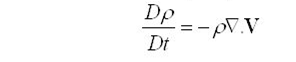
\includegraphics[width=4cm]{imgs/ciaglosc.png}
		\end{textblock}
		\begin{textblock}{4}(5.001,3.501)
			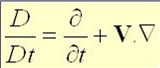
\includegraphics[width=2cm]{imgs/ciaglosc2.png}
		\end{textblock}
		\begin{textblock}{10}(0.501,5.501)
			Równania Naviera-Stokesa (czyli równania pędu):
			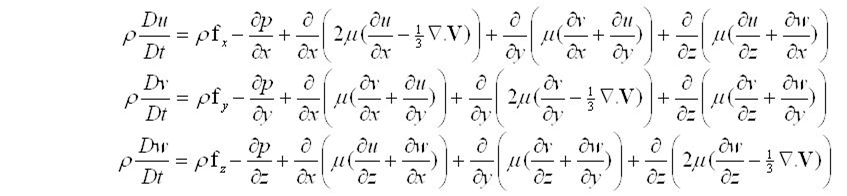
\includegraphics[width=10cm]{imgs/NS.png}
		\end{textblock}
		\begin{textblock}{13}(0.501,10.501)
			Równanie energii przepływu lepkiego:
			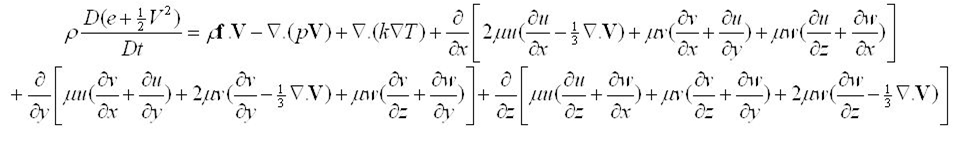
\includegraphics[width=13cm]{imgs/energia.png}
		\end{textblock}
	\end{frame}
	
	
	\section{Wykorzystywane metody i ich zastosowanie}
	\subsection{Wektory i wartości własne}
	
	\begin{frame}
		\begin{textblock}{13}(5.501,1.001)
			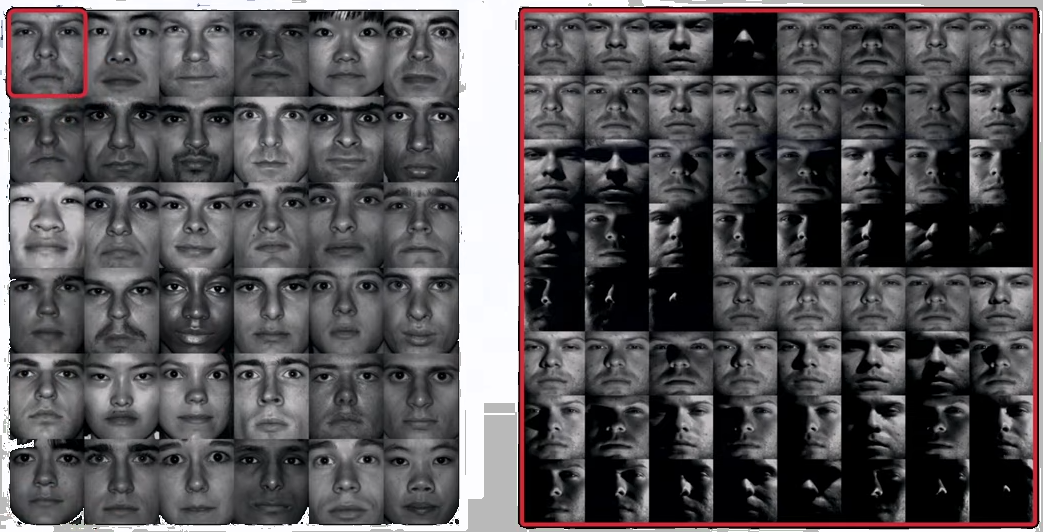
\includegraphics[width=10cm]{imgs/faces2.png}
		\end{textblock}
		\begin{textblock}{13}(0.501,7.201)
			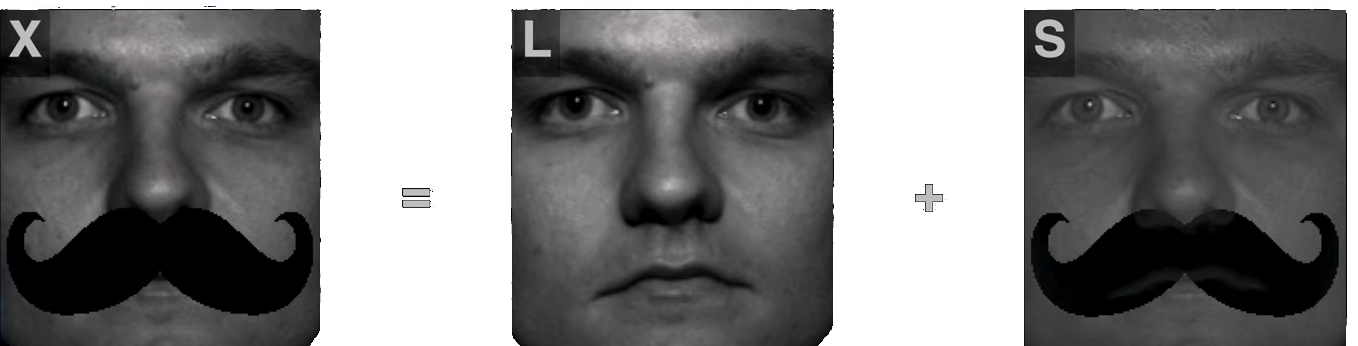
\includegraphics[width=12cm]{imgs/faces1.png}
		\end{textblock}
	\end{frame}

	\begin{frame}{Wektory i wartości własne}
		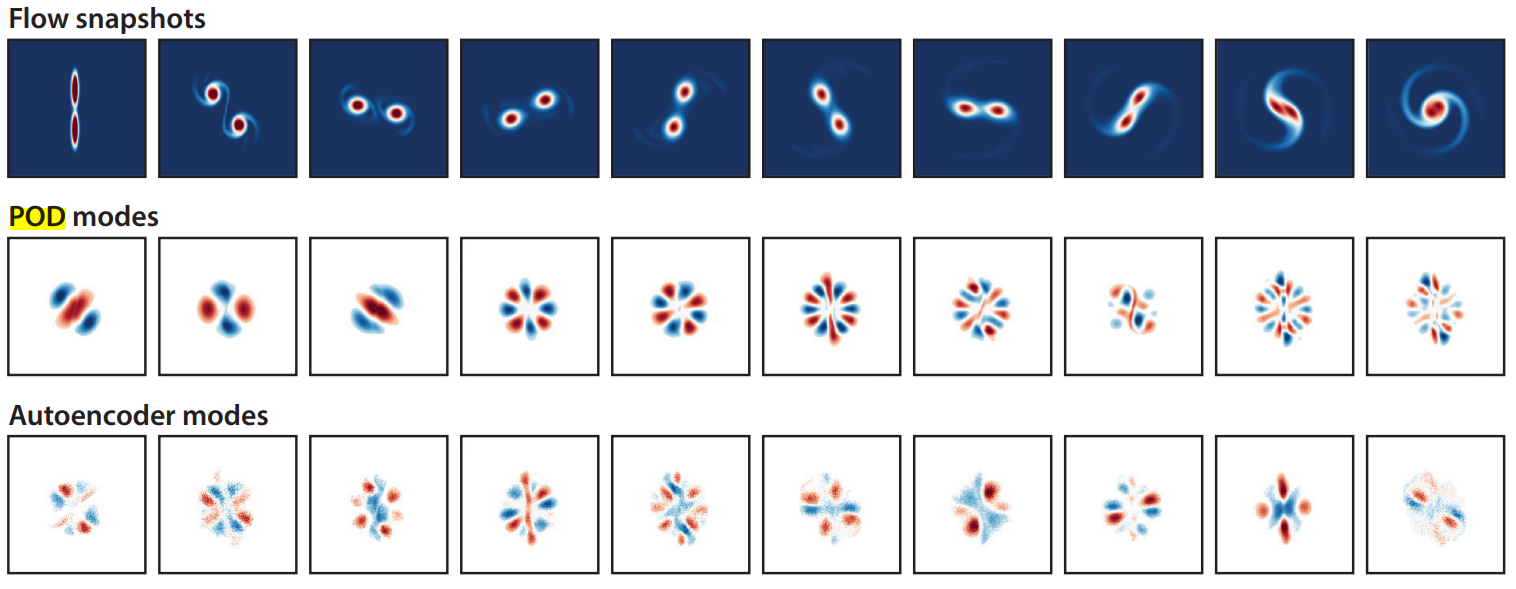
\includegraphics[width=14cm]{imgs/pca_pod.png}
	\end{frame}
	
	\begin{frame}
		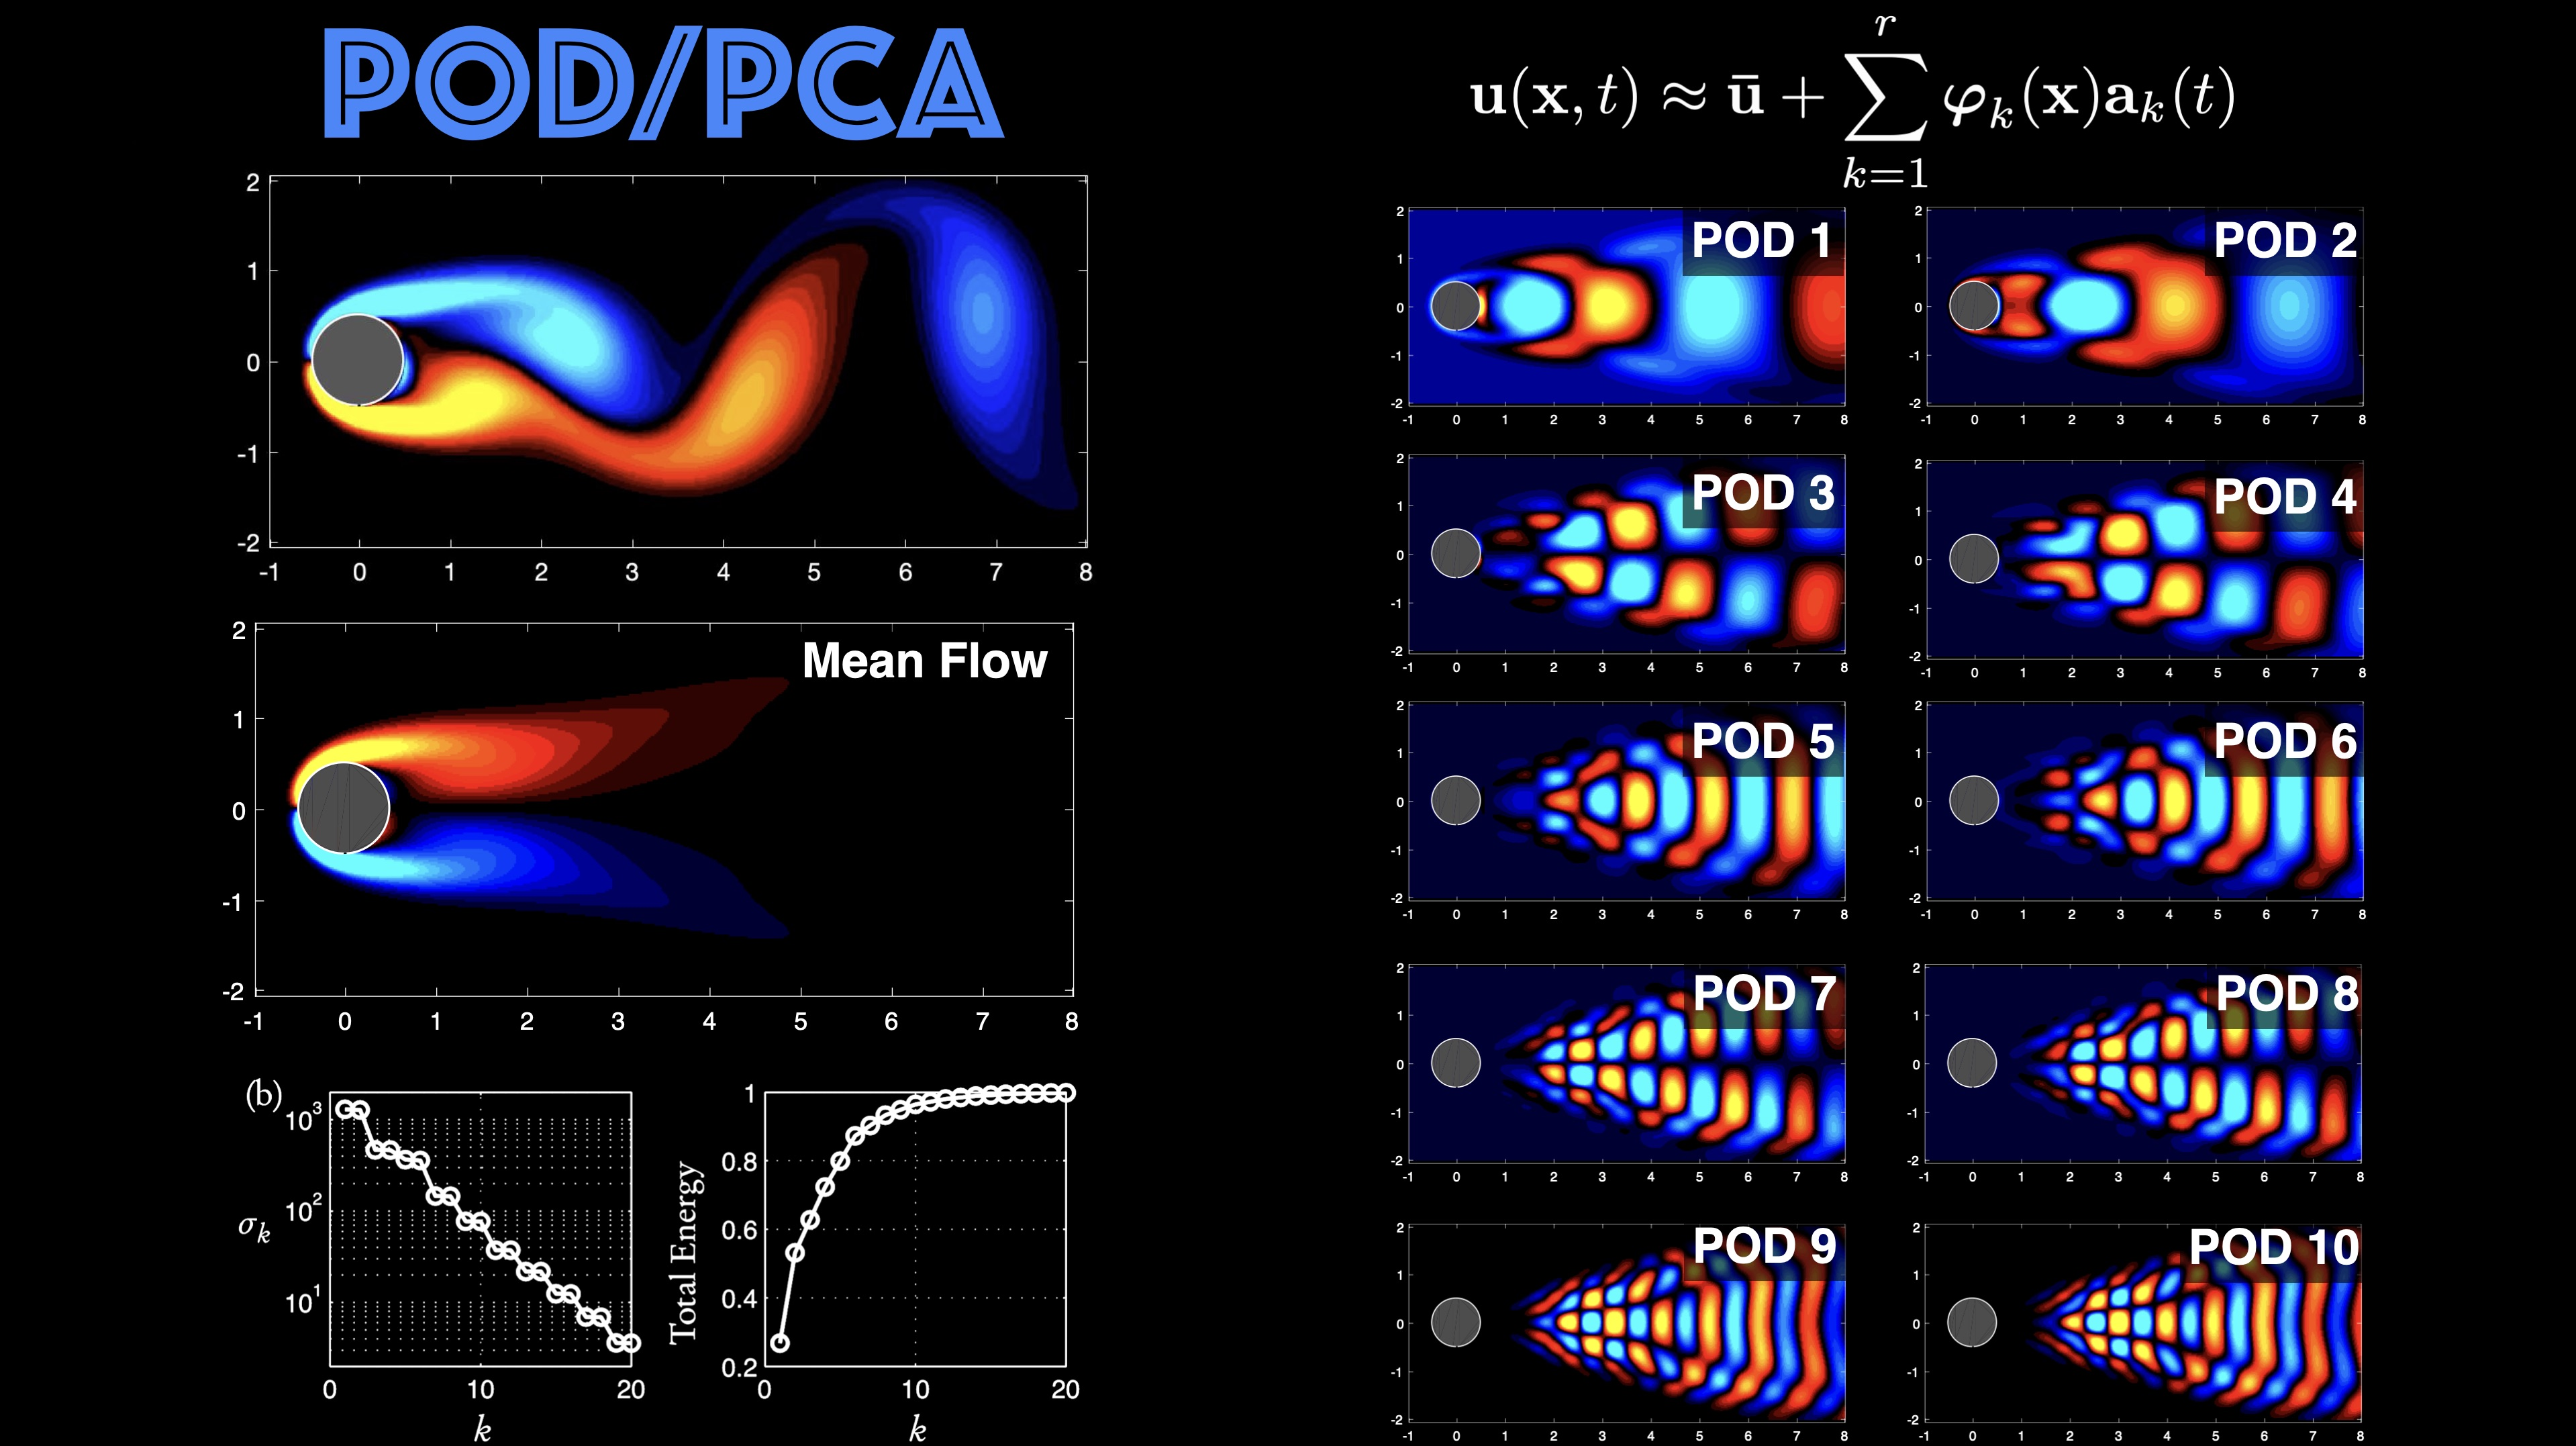
\includegraphics[width=14cm]{imgs/patterns.jpg}
	\end{frame}

	\subsection{PCA and POD}
	\begin{frame}{Principal Component Analisis and Proper Orthogonal Decomposition}
		\begin{textblock}{13}(6.001,2.001)
			Sposób na otrzymanie wartości i wektorów własnych:
			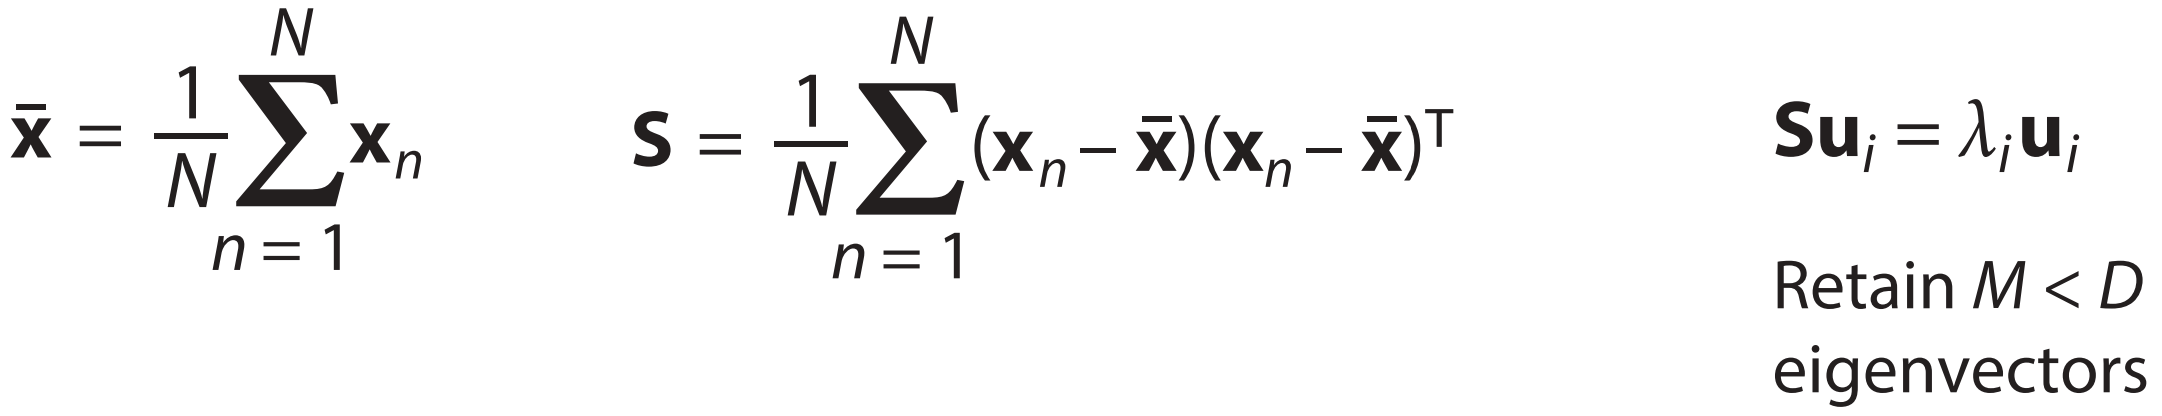
\includegraphics[width=10cm]{imgs/PCAandPODequation.png}
		\end{textblock}
		\begin{textblock}{13}(1.501,5.001)
			Shallow autoencoder\qquad \qquad \qquad \qquad Deep autoencoders
			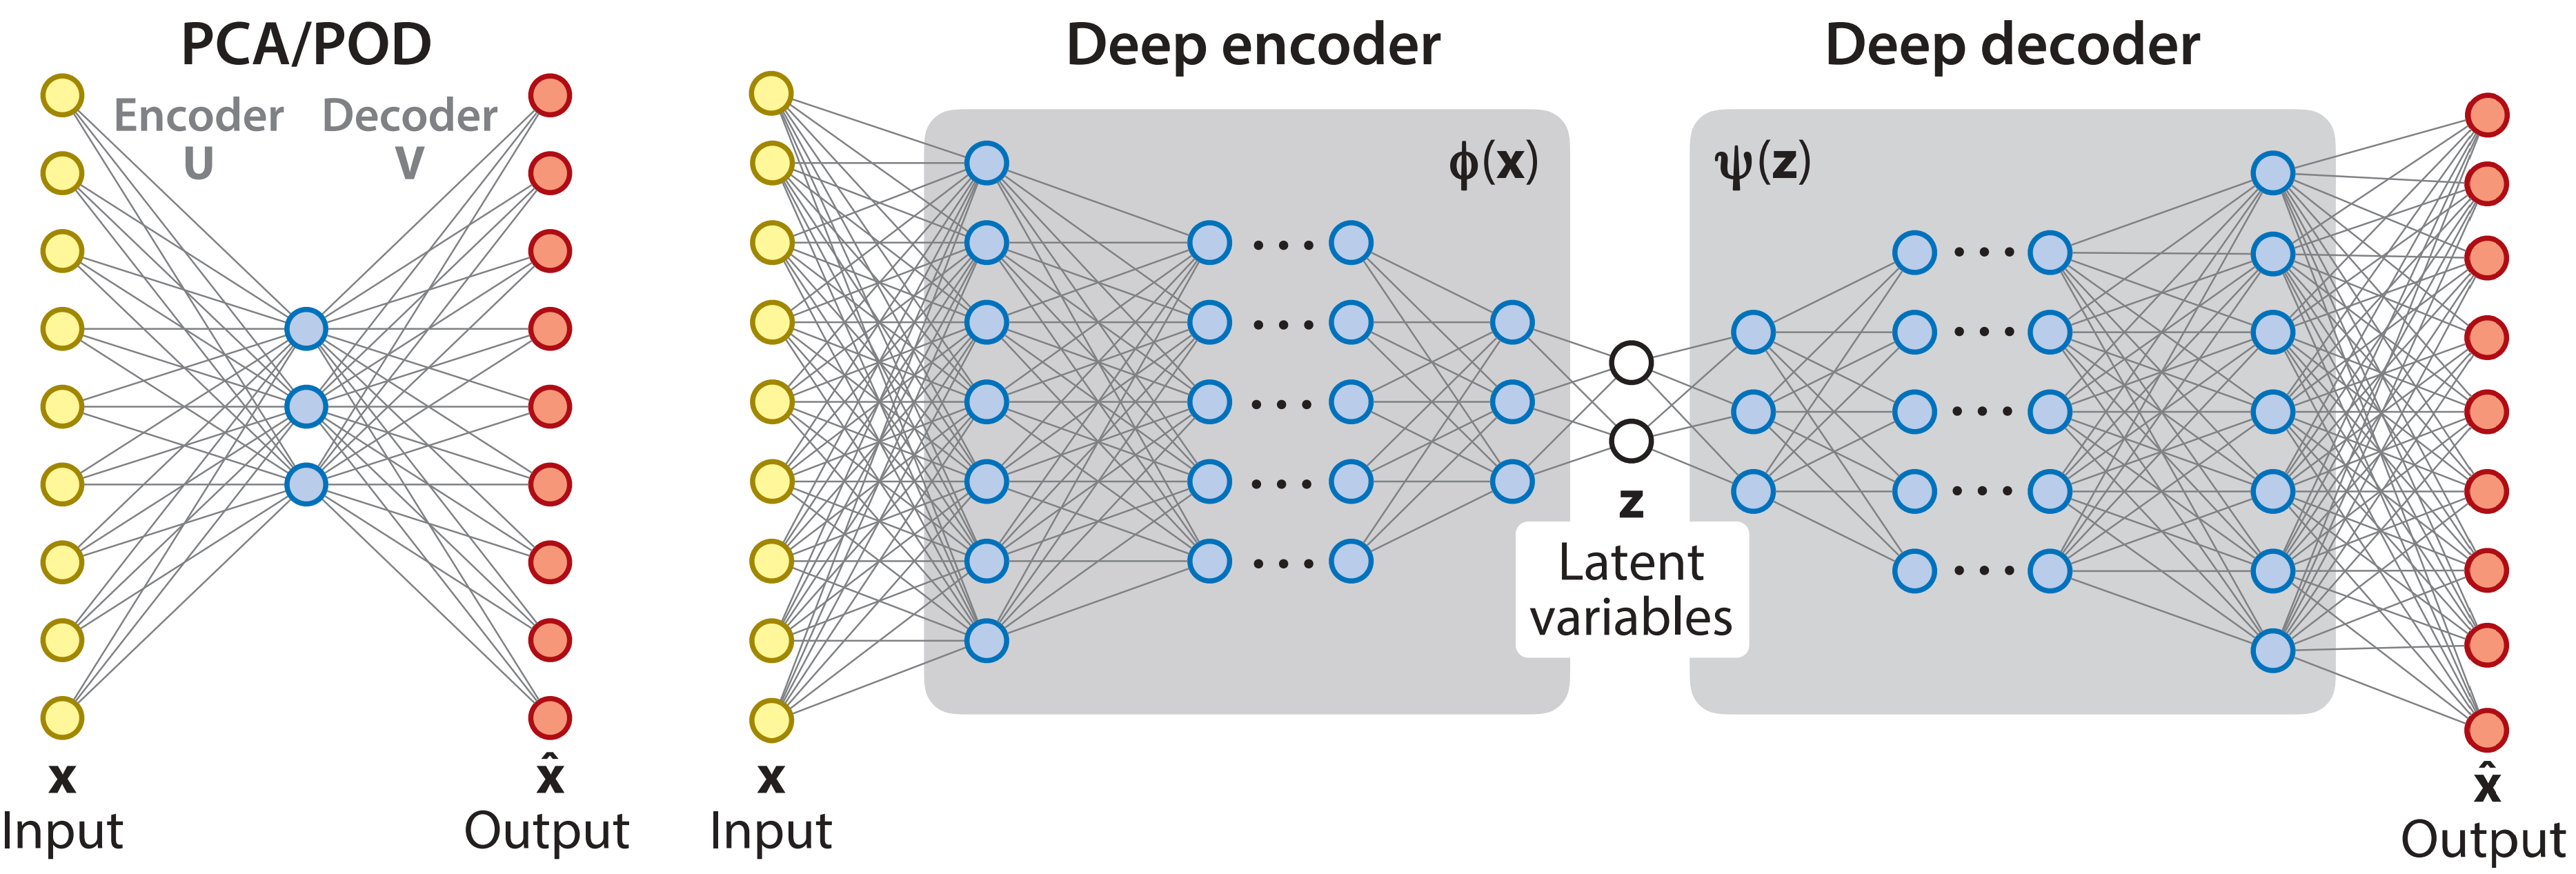
\includegraphics[width=13cm]{imgs/PCAandPOD.png}
		\end{textblock}
	\end{frame}


\begin{frame}
	\begin{textblock}{13}(3.501,1.001)
		Oderwanie warstwy przyściennej w kanale rozszerającym się
		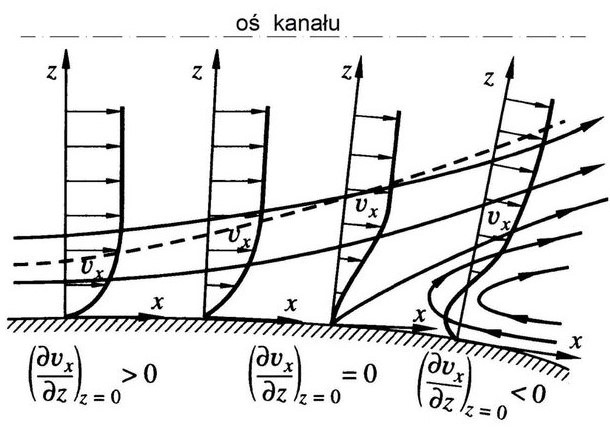
\includegraphics[width=10cm]{imgs/oderwanie.png}
	\end{textblock}
\end{frame}

\begin{frame}
	\begin{textblock}{13}(4.501,2.001)
		Profil warstwy przyściennej obliczony autoenkoderem
		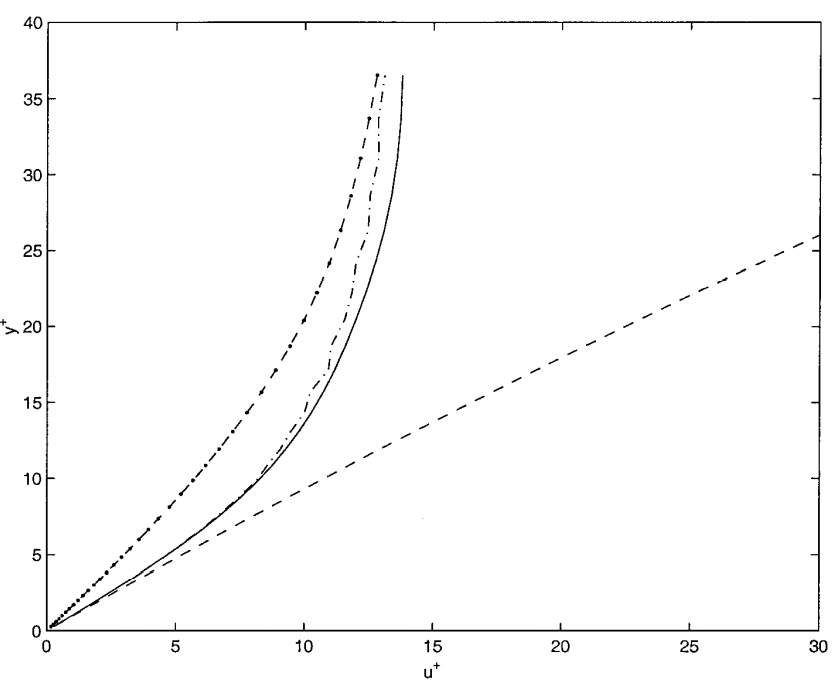
\includegraphics[width=8cm]{imgs/velocity2.png}
	\end{textblock}
\end{frame}

\subsection{Robust POD/PCA}
\begin{frame}{Robust POD/PCA}
	\begin{textblock}{13}(2.101,1.701)
	\qquad \qquad \qquad \qquad \qquad Particle Image Velosimetry
	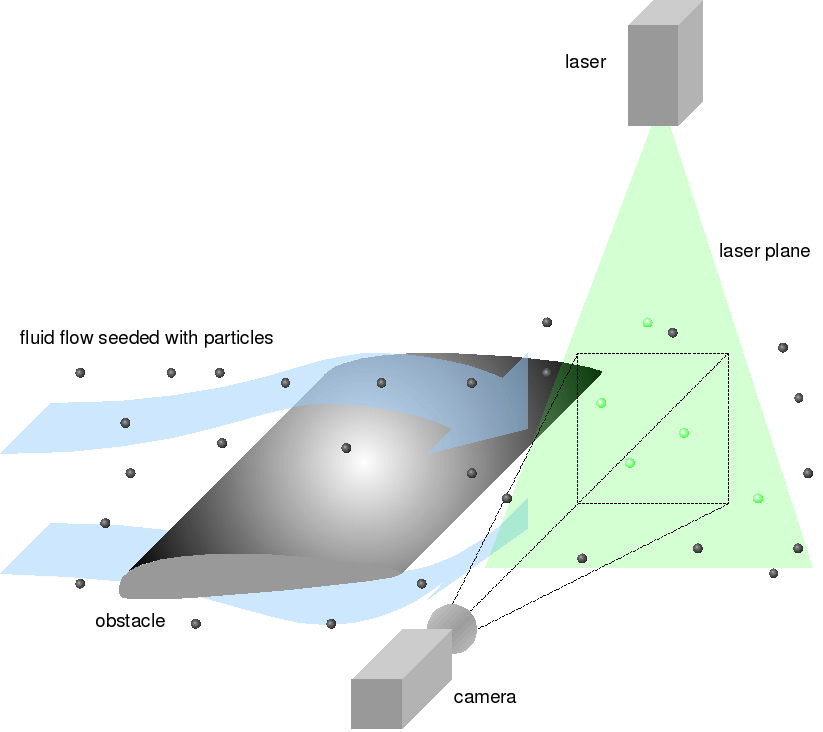
\includegraphics[width=8cm]{imgs/piv.png}
	\end{textblock}
\end{frame}

\begin{frame}{Robust POD/PCA}
\begin{textblock}{13}(5.501,1.001)
	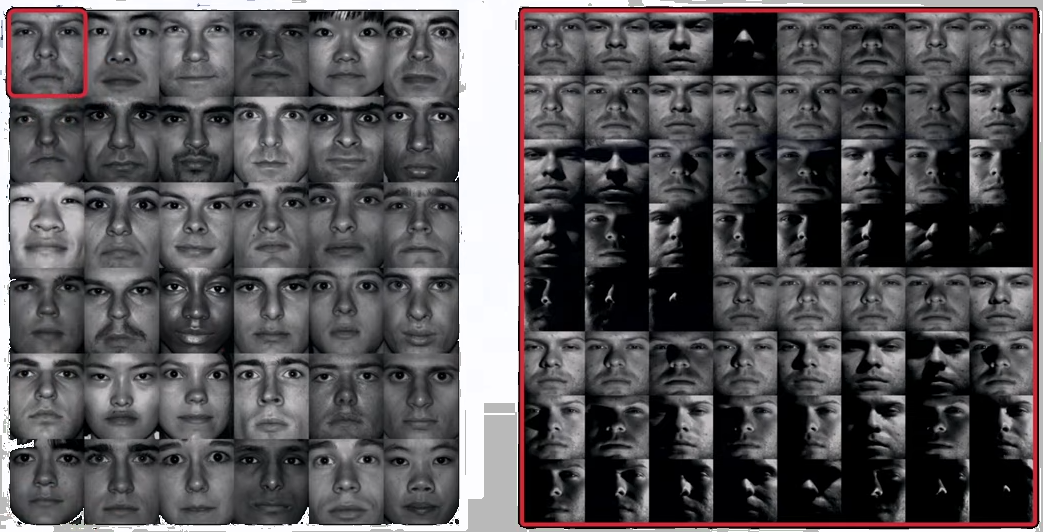
\includegraphics[width=10cm]{imgs/faces2.png}
\end{textblock}
\begin{textblock}{13}(0.501,7.201)
	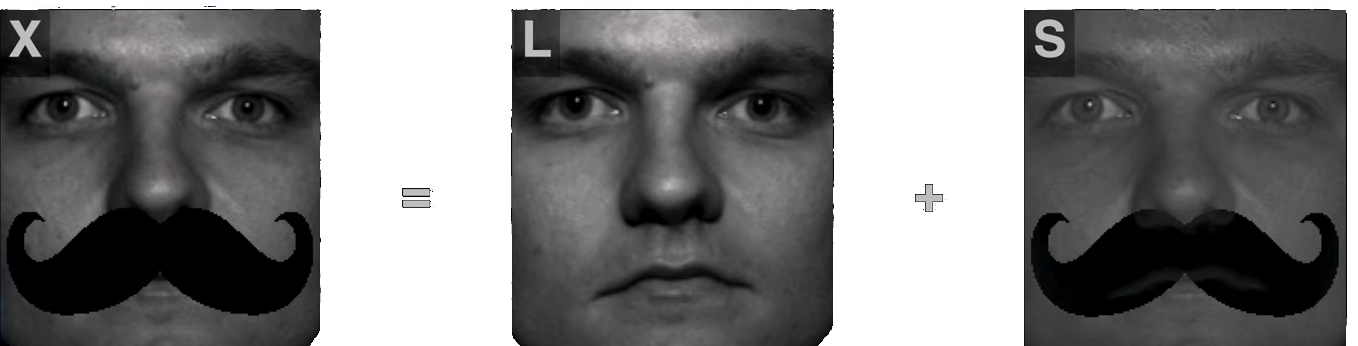
\includegraphics[width=12cm]{imgs/faces1.png}
\end{textblock}
\end{frame}

\begin{frame}{Robust POD/PCA}
	\begin{textblock}{13}(0.501,3.001)
		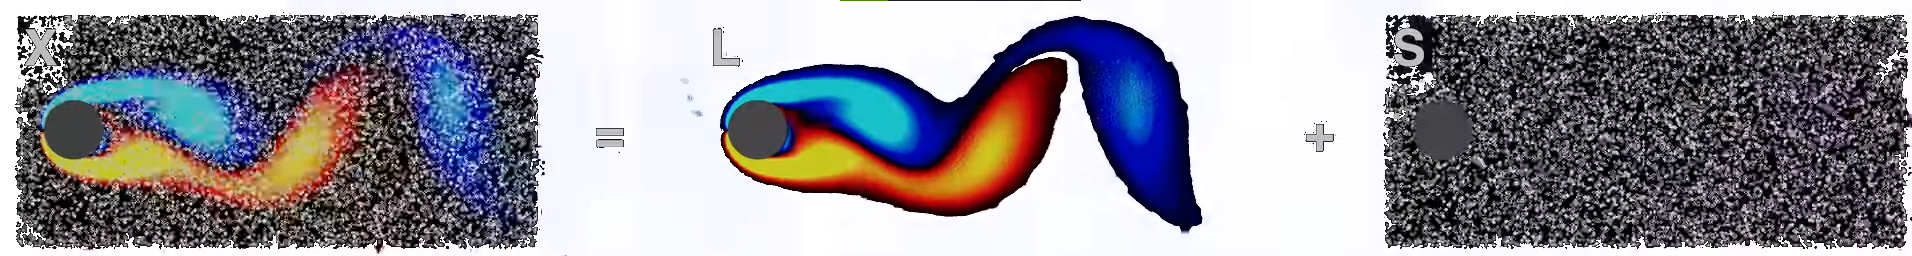
\includegraphics[width=15cm]{imgs/eigenflow.png}
	\end{textblock}
	\begin{textblock}{13}(1.001,7.001)
		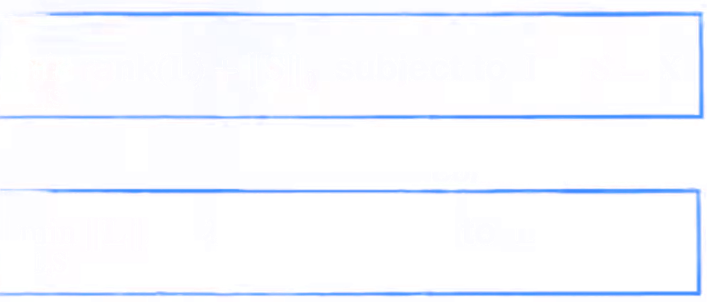
\includegraphics[width=7cm]{imgs/eigenflow2.png}
	\end{textblock}
	\begin{textblock}{13}(8.501,7.001)
		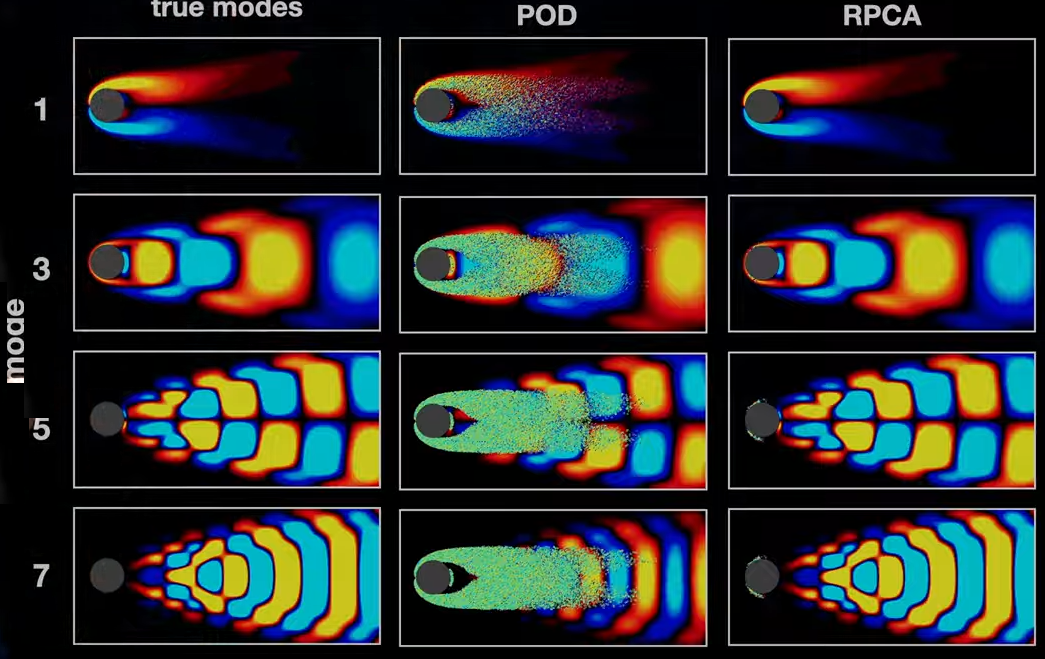
\includegraphics[width=7cm]{imgs/rpca.png}
	\end{textblock}
\end{frame}

%	\subsection{Recursive Neural Networks}
%	\begin{frame}{Recursive Neural Networks}
%		a
%	\end{frame}
%	
%	\subsection{Generative Adversarial Network}
%	\begin{frame}{Generative Adversarial Network}
%		a
%	\end{frame}
%
%	
%	\subsection{Porównanie dokładności predykcji i kosztu czasowego uczenia}
%	\begin{frame}{Porównanie dokładności predykcji i kosztu czasowego uczenia}
%		\begin{table}
%			\centering
%			\arrayrulecolor{white}
%			\color[HTML]{303030}
%			{\rowcolors{3}{blue!60!yellow!20}{blue!30!yellow!5}
%				\begin{center}
%					\begin{tabular}{ |c|s|s|s|  }
%						& \multicolumn{3}{|t|}{Koszt\ czasowy\ uczenia\ się} \\
%						% \rowcolor[HTML]{4bb5d2}
%						& \cellcolor[HTML]{82E0AA} Niski & \cellcolor{red!40!yellow!70} Średni & \cellcolor[HTML]{EC7063} Wysoki \\
%						\cellcolor[HTML]{F9E79F}  & - & - &  \\
%						\cellcolor[HTML]{F9E79F} Niska dokładność & - & - &\\
%						\cellcolor[HTML]{F9E79F}  & RNNs & - &\\
%						\cellcolor[HTML]{BB8FCE}  & - & - & CMA-ES \\
%						\cellcolor[HTML]{BB8FCE} Wysoka dokładność & - & Gaussian Process &\\
%						\cellcolor[HTML]{BB8FCE}  & \cellcolor[HTML]{F7DC6F} - & - & Bayesian Inference \\
%					\end{tabular}
%					\caption{Dokładność i koszt czasowy uczenia się poszczególnych algorytmów}
%					\label{tab:template}
%				\end{center}
%			}
%		\end{table}
%	\end{frame}

	
	
	\begin{frame}
		\begin{center}
			
\includegraphics[width=5cm]{imgs/dziekuje.jpg}
		\end{center}
	\end{frame}
	
	\begin{frame}[allowframebreaks]
		\frametitle{References}
\begin{thebibliography}{9}
	
	\bibitem{flow_image}
	Leonardo da'Vinci  \textit{\href{https://images.slideplayer.com/26/8393980/slides/slide_5.jpg}{Flow}}.
	
	\bibitem{datacamp}
	Steven L. Brunton, Bernd R. Noack, and Petros Koumoutsakos
	\textit{\href{https://www.annualreviews.org/doi/abs/10.1146/annurev-fluid-010719-060214}{Machine Learning for Fluid Mechanics}}. 
	
%	\bibitem{datacamp}
%	Ilhan, Hamza Osman, and Mehmet Fatih Amasyali. 
%	\textit{Active Learning as a Way of Increasing Accuracy.}. 
%	\texttt{International Journal of Computer Theory and Engineering 6, no. 6 (2014): 460.}
%	
\end{thebibliography}
	\end{frame}
	


	
\end{document}
